\documentclass[a4paper,11pt,oneside]{report}
% Options: MScThesis, BScThesis, MScProject, BScProject, lablogo
\usepackage[MScThesis]{EPFLreport}

% Needs to be in this file if we want autocompletion to work
\addbibresource{thesis.bib}

\title{Document representation for end to end encrypted search and machine learning}
\author{Florian Singer}
\epflsupervisor{Prof. Serge Vaudenay}
\companysupervisor{Nicolas Casademont}

%\dedication{...}
%\acknowledgments{...}

\begin{document}
\maketitle
%\makededication
%\makeacks

\begin{abstract}
% The abstract serves as an executive summary of your project.
% Your abstract should cover at least the following topics, 1-2 sentences for each: what area you are in, the problem you focus on, why existing work is insufficient, what the high-level intuition of your work is, maybe a neat design or implementation decision, and key results of your evaluation.
[...]
\end{abstract}

\maketoc

% Memo: shortcuts VSCode
% Jump from code to pdf: Ctrl+Alt+J
% Jump from pdf to code: Ctrl+Click

%%%%%%%%%%%%%%%%%%%%%%
\chapter{Introduction}
%%%%%%%%%%%%%%%%%%%%%%

% The introduction is a longer writeup that gently eases the reader into your thesis. 
% Use the first paragraph to discuss the setting.
% In the second paragraph you can introduce the main challenge that you see.
% The third paragraph lists why related work is insufficient.
% The fourth and fifth paragraphs discuss your approach and why it is needed.
% The sixth paragraph will introduce your thesis statement. Think how you can distill the essence of your thesis into a single sentence.
% The seventh paragraph will highlight some of your results
% The eights paragraph discusses your core contribution.

% This section is usually 3-5 pages.

The boom of artificial intelligence and machine learning seen in the past decade has had significant impact on societies, with the rise of recommender systems, image recognition software and large-scale advertisement platforms, to name a few. These advances can be beneficial, but they come with many risks and challenges that are often disregarded for the sake of short-term profit.

One of the main challenge is related to the sensitivity of the data used in these systems. As many different actors are usually participating in the training and usage of a machine learning (ML) model, the data providers need to place a high level of trust in the other actors.

This trust can be achieved through legal bindings, but only technological safeguards can provide real guarantees that the data will not be misused.

One of these safeguards is to hide the data with encryption. However, the mainstream cryptography of today only protects the data while in transit or at rest, and it cannot be used when performing operations on it. This limitation is fortunately lifted in a particular subset of cryptographic schemes, called homomorphic encryption (HE) schemes. These have the advantage of allowing some operations, primarily additions and multiplications, while keeping the numbers fully encrypted.

The downside of this approach is that it comes with severe performance and precision limitations, and is thus difficult to apply in the context of machine learning where computations are already gluttonous in resources. Nevertheless, this has been an active research field that has seen promising advances in the past decade [...].

The goal of this thesis is to identify, implement and evaluate the state-of-the-art solutions of homomorphically encrypted machine learning. It also aims to formalize and describe on a more granular level which steps of a machine learning algorithm can be protected using homomorphic encryption, and why.


%%%%%%%%%%%%%%%%%%%%
\chapter{Background}
%%%%%%%%%%%%%%%%%%%%

% The background section introduces the necessary background to understand your work. 
% This is not necessarily related work but technologies and dependencies that must be resolved to understand your design and implementation.

% This section is usually 3-5 pages.

%%%%%%%%%%%%%%%%%%%%%%%%
\section{Logistic regression}

Logistic regression is a simple and widely used model for classification. Given a set of $n$ training points $\mathbf{x}_i \in \mathbb{R}^d$ and the corresponding label $y_i \in \{-1,1\}$, the training phase consists of learning a vector of weights $\mathbf{w} \in \mathbb{R}^{d+1}$ minimizing the loss function:
\begin{equation}\label{eq:logistic_reg_train}
    \mathcal{L}(\mathbf{w}) = \frac{1}{n} \sum_{i=1}^{n} \log(1 + \exp(-\mathbf{z}_i^T \mathbf{w})) 
\end{equation}
where $\mathbf{z}_i = y_i \cdot (1, \mathbf{x}_i)$ for $i=1,...,n$.

A common method used to minimize the loss function is the gradient descent algorithm. It iteratively updates the weights vector by following the direction opposite to the gradient of the function:
\begin{align}\label{eq:gradient_descent}
    \mathbf{w}^{t+1} & = \mathbf{w}^t - \gamma\nabla\mathcal{L}(\mathbf{w}) \nonumber \\ 
    & = \mathbf{w}^t + \frac{\gamma}{n} \sum_{i=1}^{n} \sigma(-\mathbf{z}_i^T \mathbf{w}^t) \cdot \mathbf{z}_i
\end{align}
where $\gamma$ is the learning rate and $\sigma$ is the sigmoid function (or logistic function) defined as:
\begin{equation}\label{eq:sigmoid}
    \sigma(x) = \frac{1}{1 + e^{-x}}
\end{equation}

Classifying a new point $\mathbf{x}$ can be done as follows:
\begin{equation}\label{eq:logistic_reg_pred}
    y = 
    \begin{cases}
        1, & \text{if } (1, \mathbf{x}) \cdot \mathbf{w} > 0 \\
        -1, & \text{otherwise} \\
    \end{cases}
\end{equation}

%%%%%%%%%%%%%%%%%%%%%%%%
\section{Neural networks}

Neural networks are defined as a succession of \emph{layers}, each consisting of operations on a set of input neurons, which are typically real numbers.

Basic networks make use of \emph{fully connected} (or linear) layers, which are defined as such for an input vector $\mathbf{x} \in \mathbb{R}^d$, a weights matrix $W \in \mathbb{R}^{k \times d}$ and a bias vector $\mathbf{b} \in \mathbb{R}^k$:

\begin{equation}\label{eq:linear_layer}
    h^{\mathrm{linear}}(\mathbf{x}) = W \mathbf{x} + \mathbf{b}
\end{equation}

Usually, a non-linear \emph{activation function} is applied to the output in order to learn more complex decision boundaries. The most common is $\mathrm{ReLU}(x) = \max(0, x)$, but the sigmoid (\autoref{eq:sigmoid}) or the hyperbolic tangent function are also often used.

The training phase is made of two main steps. First, a data point (or a batch of data points) is evaluated successively through the layers, in what we call the forward pass. Then, we perform a gradient descent by computing the gradients at each neuron and by updating the weights, starting from the end of the network. This is called the backward pass.

Once the model is trained, it can be used to classify new data points. For this operation, only the forward pass is required.

\subsection{Convolutional neural networks}

In many practical cases, particularly for image recognition, the input dimensions can be quite big. This is a problem, because a linear layer connects every input neuron with every output neuron. In order to improve performance and better exploit the spatiality properties of pixels in images, we can limit the connections of a pixel to its neighborhood. This amounts to applying a convolution.

For an image $x \in \mathbb{R}^{c \times h \times w}$ with $c$ channels, a height of $h$ and a width of $w$ pixels, a 2D convolutional layer is defined as follows for each output channel $i$:
\begin{equation}\label{eq:conv2d_layer}
    h_i^{\mathrm{conv2d}}(x) = b_i + \sum_{k=1}^{c} w_{i, k} \star x_{k}
\end{equation}
where $b_i$ is the bias, $w_i \in \mathbb{R}^{c \times k_1 \times k_2}$ is the kernel and $\star$ is the 2D cross-correlation operation.

Another important type of layer is the \emph{pooling} layer, that will aggregate a neighborhood of neurons into one value. The type of aggregate is usually a \emph{max} operation or an \emph{average}.

The traditional architecture of a convolutional neural network starts with an alternate of convolutions, activation functions and pooling layers. Then, the input is flatten into one dimension and feeded to a sequence of fully connected layers.


%%%%%%%%%%%%%%%%%%%%%%%%
\section{Homomorphic encryption}

The basic idea of homomorphic encryption is to allow computations on encrypted data, which is not possible with most modern schemes used today. This problem has been studied for many years, with the first schemes supporting only one type of operation, such as the Paillier \cite{paillier_public-key_1999} cryptosystem supporting homomorphic additions. 

The main revolution of the field was due to Gentry \cite{gentry_fully_2009} in 2009, when he presented a blueprint for constructing fully homomorphic encryption schemes. Fully homomorphic schemes support two types of primitive operations, typically additions and multiplications, and can evaluate arithmetic circuits of arbitrary depth thanks to a \emph{bootstrapping} procedure.

From this blueprint were born many cryptosystems that are used today, such as BGV \cite{brakerski_leveled_2012}, BFV \cite{fan_somewhat_2012}, or CKKS \cite{cheon_homomorphic_2016, cheon_full_2018}. The former two work with vectors of integers, and the latter works with vectors of complex numbers.

Here is a list of the basic operations available with CKKS:
\begin{itemize}
    \item \texttt{KeyGen}: Generate a public key and a private key.
    \item \texttt{Encode}: Encode a vector of complex numbers into a plaintext, which is a polynomial in the ring $R = \mathbb{Z}[X]/(X^N + 1)$.
    \item \texttt{Decode}: Decode a plaintext back into a vector.
    \item \texttt{Encrypt}: Encrypt a plaintext with the public key into an element of $R_q^2$ where $R_q = R/qR$ is a set of polynomials with coefficients modulo $q$.
    \item \texttt{Decrypt}: Decrypt a ciphertext with the private key.
    \item \texttt{Add}: Pairwise addition of two ciphertexts, or one ciphertext and one plaintext.
    \item \texttt{Multiply}: Pairwise multiplication of two ciphertexts/plaintext.
    \item \texttt{Rotate}: Permute the elements in a ciphertext by shifting them by $k$ positions.
    \item \texttt{Relinearize}: After a multiplication, the resulting ciphertext will be in $R_q^3$ and will continue to grow after each multiplication. Relinearization is used to bring it back to $R_q^2$ and facilitate decryption.
    \item \texttt{Rescale}: Rounding operation performed to maintain the size of a ciphertext after a multiplication.
    \item \texttt{Bootstrap} \cite{nielsen_bootstrapping_2018}: Refresh a ciphertext once it reached its maximum number of operations.
\end{itemize}

To initialize the context, some parameters need to be set:

\emph{Ring degree} [...]

\emph{Moduli chain} [...]

The \emph{scale} of the plaintext, determining how many bits are consumed during a rescale operation.

\emph{Error distribution} [...]



%%%%%%%%%%%%%%%%
\chapter{Design}
%%%%%%%%%%%%%%%%

% Introduce and discuss the design decisions that you made during this project.
% Highlight why individual decisions are important and/or necessary. 
% Discuss how the design fits together.

% This section is usually 5-10 pages.

%%%%%%%%%%%%%%%%%%%%%%%%
\section{Threat model}

In order to justify the use of cryptography as a mitigation, it is useful to identify and formalize the potential threats that a machine learning system can face. This also helps us to understand how this type of mitigation can be bypassed.

\subsection{Data-flow diagram}

\begin{figure}[t]
    \centering
    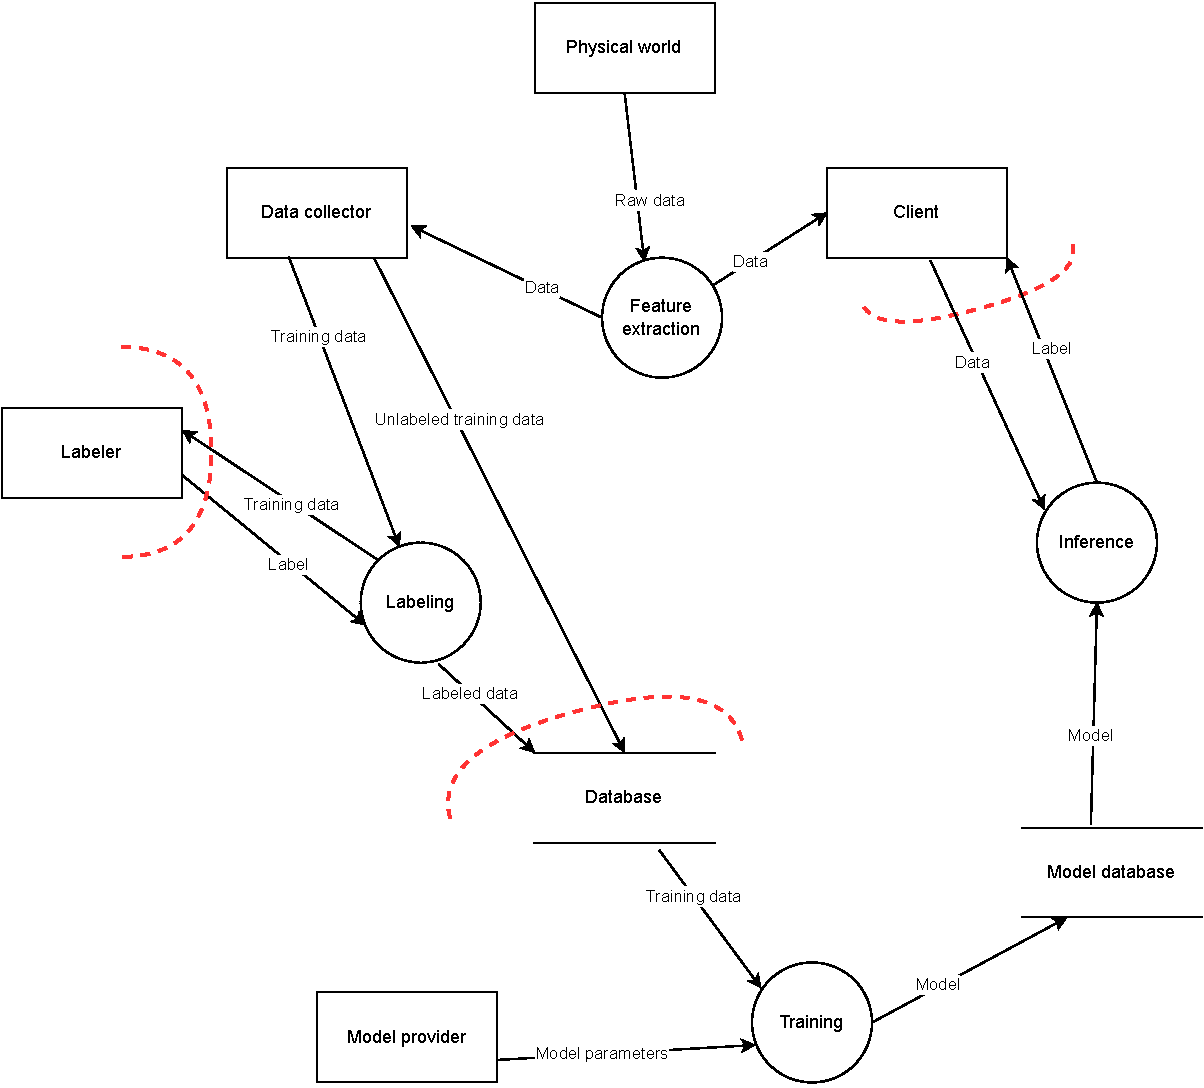
\includegraphics[width=\textwidth]{figures/dataflow-ml.pdf}
    \caption{Dataflow diagram for a general ML system.}
    \label{fig:dataflow}
\end{figure}

In order to better visualize how a machine learning system looks like, \autoref{fig:dataflow} attempts to model the data flow in a general case. This diagram could be refined in more concrete applications. For instance, the model provider and the data collector may be the same entity, which would remove a trust boundary. Another gray area is the feature extraction process that can happen in different ways: it could be done directly on the client and the data collector, or it could rely on an external service controlled by the model provider.

Thus, in this case, the goal of this diagram is to be a tool for identifying the threats, rather than an exhaustive reference.

\subsection{Threats}\label{sec:threats}

From surveys of the ML security literature \cite{liu_survey_2018, rigaki_survey_2021}, we can identify many types of threats:

\begin{itemize}
    \item Poisoning attacks
    \item Evasion/impersonation attacks
    \item Data ordering attacks
    \item Model extraction attacks
    \item Membership inference attacks
    \item Inversion attacks
    \item Attribute inference attacks (leakings features of samples)
    \item Property inference attacks (leaking features of datasets)
\end{itemize}

In many cases, the attacker needs to influence the training process by injecting or modifying the input data.

Let us take the example of a classification model based on textual data from documents. To carry out a poisoning attack, an adversary could create spam documents with uncommon words. This will reduce the utility of the system by replacing useful words in the feature vector. If the system lets adversaries define the labels, the model can also be poisoned with incorrect labels. This type of attack can be detected with the help of another model specialized in anomaly detection.

For evasion or impersonation attacks, the attack vector is the same but it involves carefully crafted inputs in order to produce a specific result. 

In the same vein, data ordering attacks aim to reduce the utility or even bias the model by putting some data points first \cite{shumailov_manipulating_2021}. This could be used to introduce racist or sexist biases, for instance. Thus, it is important to shuffle the training data properly.

If the attacker has unlimited access to the prediction results, it may be possible to reconstruct and steal an approximation the model (model extraction attack). The typical type of adversary carrying out this attack could be a competitor unwilling to dedicate the resources necessary for training a model from scratch.

In the case of membership inference attacks, inversion attacks, attribute and property inference attacks, the goal is to reconstruct part of the training dataset. This can either be general or target a single individual. To be successful, the attacker sometimes needs to do data poisoning \cite{hidano_model_2017}, or needs access to additional information, such as confidence levels or auxiliary datasets \cite{fredrikson_model_2015, wang_variational_2022}.


%%%%%%%%%%%%%%%%%%%%%%%%
\section{Secure training}\label{sec:secure_training}

In addition to the threats that we identified in \autoref{sec:threats}, another one is that external actors, such as hackers or cloud providers, could observe the training process and exfiltrate the data. A potential defense mechanism is to train the model on homomorphically encrypted data.

In our case, we assume that the whole training data matrix is encrypted with the same key. The holder of this key is both the model owner and the data owner. The data should be encrypted in a secure enclave before sending it to the training service. 

If the data comes from external data owners and should not be visible to the model owner, we can design a protocol using multi-party homomorphic encryption. However, this feature is not available in many HE libraries.

If we distinguish the client (data and model owner) and the server (computing power provider), the steps of an encrypted training procedure can be described as follows:
\begin{enumerate}
    \item Client: initialize the keys and encrypt the data. Send the encrypted data and other objects or parameters required for homomorphic computations (e.g. rotation keys, relinearization keys).
    \item Server: do the training. Send back the encrypted weights.
    \item Client: decrypt the weights.
\end{enumerate}

As training can be a fairly complex and resource-intensive process, it is wise to start with a simple classification model. Logistic regression models are simple and have been extensively studied as part of the 2017 iDASH secure genome analysis competition. The winning solution has been proposed by Kim et al. ~\cite{kim_logistic_2018}. This will be the basis of our implementation.


%%%%%%%%%%%%%%%%%%%%%%%%
\section{Private inference}

In the case of an inference service provided by a model owner to a client, another threat is that the client's data can be abused. Even with a privacy policy, the client has no technical guarantee that this data will not be shared, stolen, or used for different purposes. As opposed to the attacks mentioned in \autoref{sec:threats}, this threat is independent of the ML model and involves only the data. Homomorphic encryption aims to reduce this risk, thus improving the overall trust in the system.

There are two approaches to this problem. In both cases, we assume that a model has been trained beforehand. 

In the most common approach, the client encrypts the data and sends it to the inference service, who learns nothing about the data and the inference result.

In the second approach, the weights of the model are encrypted and sent to the client. This requires an additional round-trip of communications for the decryption step, which can reveal the inference result to the service if no precautions are made. In addition, the architecture of the model must be revealed to the client, which incurs the risk of it being stolen and retrained from scratch by a competitor. Due to these limitations, we will focus on the first approach, but the runtime estimates should not differ too much between the two.

This time, if we consider the client to be the data owner and the server to be the model owner, the steps are very similar to \autoref{sec:secure_training}:
\begin{enumerate}
    \item Client: initialize the keys and encrypt the data. Send the encrypted data and the required keys.
    \item Server: do the inference. Send back the result.
    \item Client: decrypt the result.
\end{enumerate}

Note that the inference step can also be delegated to an external cloud provider without risks of compromising the data.

Because inference requires much less resources than training, we can look at more complex models. As neural networks are extremely popular nowadays, a deep learning framework compatible with encrypted data has many use-cases.

\subsection{Packing}

This problem, especially for the special case of neural networks, has already been widely studied. One of the first solution was proposed by Dowlin et al. \cite{dowlin_cryptonets_2016} in 2016. One of the particularity of their approach is that they pack the $n$ pixels of an image into $n$ different ciphertexts. This is very efficient when batching multiple images (by putting the pixels of the first image in the first slots, the pixels of the second image in the second slots, etc) but results in a lot of wasted if only one image needs to be evaluated. In the following, we will call this method \emph{pixelwise packing}.

An alternative is to pack the pixels of an image one after the others in the same ciphertext. This results in a more efficient use of space when doing few inferences. For simplicity, we assume that the number of pixels fit into a single ciphertext. We also separate each channel into its own ciphertext. For this reason, we call this method \emph{channelwise packing}.

Both methods have their own trade-offs that highly depend on the architecture of the network. They are evaluated side by side in \autoref{chap:evaluation}.

["If we look at the theoretical complexity..." Detail the trade-off]

[Check: has channelwise packing been described in the literature?]


%%%%%%%%%%%%%%%%%%%%%%%%
\chapter{Implementation}
%%%%%%%%%%%%%%%%%%%%%%%%

% The implementation covers some of the implementation details of your project.
% This is not intended to be a low level description of every line of code that you wrote but covers the implementation aspects of the projects.

% This section is usually 3-5 pages.

%%%%%%%%%%%%%%%%%%%%%%%%
\section{Backends}

There are multiple HE libraries providing the CKKS scheme. Most of them are implemented in \texttt{C++}, such as SEAL \cite{microsoft_corporation_microsoft_2022}, Palisade \cite{palisade_palisade_2022} or HEAAN \cite{cryptolab_inc_heaan_2022}, but Lattigo \cite{tune_insight_sa_lattigo_2022} is implemented in Golang. A more complete survey and comparison of the different libraries can be found in \cite{viand_sok_2021}.

Each of these libraries has its own particularities, as there is not yet a complete standard for homomomorphic encryption (although the work has been started in \cite{albrecht_homomorphic_2021}). In the next subsections, we will introduce the ones that have been used in this project.

Despite these differences, we implemented a higher abstraction to unify the usage of these libraries, and to provide a more intuitive API for non-expert programmers. Thanks to this, the ML algorithms can be implemented independently of the backend. The set of available primitives is slightly reduced, because the relinearization and rescaling operations are performed automatically when necessary.

One of the requirements of the project was to code in Python. This means that our implementation needs bindings to use these libraries.

\subsection{PALISADE}

PALISADE is a widely used open-source library written in \texttt{C++}. It provides incomplete bindings for Python, but we can extend them as needed. 

In its basic usage, the library creates a context from a set of parameters and stores the keys needed for the evaluation (rotation keys, etc). It is slightly higher-level than other libraries by default, e.g., it rescales ciphertexts automatically. It also provides a wide set of utility functions, such as polynomial evaluation.

Multi-party HE is supported, but not bootstrapping.

\subsection{SEAL}

SEAL, developed by Microsoft, is one of the most popular libraries. A complete set of Python bindings are already available \cite{hugang_seal-python_2022}.

It offers finer grained initialization parameters and a lower-level API (e.g., we need to set the moduli size at each level, and rescaling needs to be done manually).

It does not offer bootstrapping, nor a multi-party version.

\subsection{Plaintext}

When dealing with ciphertexts, it is extremely useful to have a cleartext pipeline that can be inspected for easier debugging. It can also be used to evaluate the cost of translating an algorithm to a homomorphic-encryption-friendly version, independently of the cost of encryption. 

For this backend, we used \texttt{numpy} vectors to represent the ciphertexts.

%%%%%%%%%%%%%%%%%%%%%%%%
\section{Logistic regression}

[Matrix packing, padding]


%%%%%%%%%%%%%%%%%%%%%%%%
\section{Neural network}

[Layers are defined with pytorch. Training is done with pytorch. Weights are exported to a file.]

% TODO refactor the other way around
[Layers are translated to the homomorphic version if all are supported.]

[...]


%%%%%%%%%%%%%%%%%%%%%%%%
\section{Challenges}

[Crypto and ML parameters]

[No bootstrapping, but it would be interesting to compare. The problem is that few libraries implement the bootstrapping operation]

[Security level]

[Scale]

[Library-specific problems, standardization]



%%%%%%%%%%%%%%%%%%%%
\chapter{Evaluation}\label{chap:evaluation}
%%%%%%%%%%%%%%%%%%%%

% In the evaluation you convince the reader that your design works as intended.
% Describe the evaluation setup, the designed experiments, and how the experiments showcase the individual points you want to prove.
% This section is usually 5-10 pages.

%%%%%%%%%%%%%%%%%%%%%%%%
\section{Logistic regression}

\autoref{table:lr_runtime} presents the runtime at every step (encryption, training, decryption, etc) of the different logistic regression algorithms.

\begin{table}[h!]
    \begin{center}
      \caption{Runtime of each step in seconds}
      \label{table:lr_runtime}
      \pgfplotstabletypeset[
        % multicolumn names,
        col sep=comma,
        display columns/0/.style={
          column name=$ $,
          column type={l},string type},
        display columns/1/.style={
          column name=Init,
          column type={l}},
        display columns/2/.style={
          column name=Encrypt train,
          column type={l}},
        display columns/3/.style={
          column name=Train,
          column type={l}},
        display columns/4/.style={
          column name=Encrypt test,
          column type={l}},
        display columns/5/.style={
          column name=Predict,
          column type={l}},
        display columns/6/.style={
          column name=Decrypt,
          column type={l}},
        every head row/.style={
            before row={\toprule},
            after row={
                % si{\second} & \si{\second} ... \\
                \midrule
            }
        },
        every last row/.style={after row=\bottomrule},
    ]{data/lr_runtime.csv}
\end{center}
\end{table}

[Accuracy table]


%%%%%%%%%%%%%%%%%%%%%%%%
\section{Neural network}

[Benchmarks of the different versions (plaintext, palisade, seal, pytorch; pixelwise and channelwise) with the different metrics (accuracy, runtime, memory)]



%%%%%%%%%%%%%%%%%%%%%%
\chapter{Related Work}
%%%%%%%%%%%%%%%%%%%%%%

% The related work section covers closely related work. 
% Here you can highlight the related work, how it solved the problem, and why it solved a different problem. Do not play down the importance of related work, all of these systems have been published and evaluated! Say what is different and how you overcome some of the weaknesses of related work by discussing the trade-offs. Stay positive!
% This section is usually 3-5 pages.

[Kim et al.: what differences between their solution and mine]

[Dowlin et al.: other encryption scheme, how they evaluated (MNIST on a very simple network of 5 layers)]


%%%%%%%%%%%%%%%%%%%%
\chapter{Conclusion}
%%%%%%%%%%%%%%%%%%%%

% In the conclusion you repeat the main result and finalize the discussion of your project. Mention the core results and why as well as how your system advances the status quo.

[...]

\cleardoublepage
\phantomsection
\addcontentsline{toc}{chapter}{Bibliography}
\printbibliography

\end{document}
